%-----------------------------------------------------------------------
% Beginning of chapter.tex
%-----------------------------------------------------------------------
%
%  This is a sample file for use with AMS-LaTeX.  It provides an example
%  of how to set up a file for a book to be typeset with AMS-LaTeX.
%
%  This is the driver file.  Separate chapters should be included at
%  the end of this file.
%
%  ***** DO NOT USE THIS FILE AS A STARTER FOR YOUR BOOK. *****
%  Follow the guidelines in the file chapter.template.
%
%%%%%%%%%%%%%%%%%%%%%%%%%%%%%%%%%%%%%%%%%%%%%%%%%%%%%%%%%%%%%%%%%%%%%%%%

\documentclass[11pt,a4paper]{memoir}
\chapterstyle{demo}
\epigraphfontsize{\small\itshape}
\setlength\epigraphwidth{8cm}
\setlength\epigraphrule{0pt}
\epigraphfontsize{\small\itshape}
%\includeonly{preface,chap1,biblio}

%\numberwithin{section}{chapter}
%\numberwithin{equation}{chapter}

% Include macros here
%=================================================
% Packages
%=================================================

%\usepackage{fixltx2e}
\usepackage[usenames,dvipsnames]{xcolor}
%\usepackage{fancyhdr}
\usepackage{amsmath,amsfonts,amsbsy,amsgen,amscd,mathrsfs,amssymb,amscd}
\usepackage{amsthm}
\usepackage{bm}
\usepackage{url}
\usepackage[UKenglish]{babel}
\usepackage{eurosym}
\usepackage{tikz}
\usepackage{caption}
\usetikzlibrary{matrix,arrows,shapes,calc,3d}
\usepackage{tikz-3dplot}
\tdplotsetmaincoords{60}{110}
\pgfmathsetmacro{\rvec}{.8}
\pgfmathsetmacro{\thetavec}{30}
\pgfmathsetmacro{\phivec}{60}

\tikzset{mynode/.style = {
    % The shape
    circle,
    % The size
    minimum size=2pt,
    % The color
    draw=black, fill=black}
}
\tikzset{vertex/.style={shape=circle, % style for a vertex
                        minimum size=3pt,
                        fill=gray,
                        inner sep = 0pt}}  

% \usepackage{3dplot}
% \tdplotsetmaincoords{60}{110}
%\usepackage{subfig}
\usepackage{microtype}
\usepackage{enumitem}
\usepackage{listings}
\definecolor{darkblue}{rgb}{0,0,.75}

\usepackage[many]{tcolorbox}
\tcbuselibrary{listings}

\definecolor{light-gray}{rgb}{0.96,0.96,0.96}
\definecolor{kwgreen}{rgb}{0,0.5,0}
\definecolor{cogreen}{rgb}{0.25,0.5,0.5}
\definecolor{mygreen}{rgb}{0,0.5,0.125}
\definecolor{equalsign}{rgb}{0.66,0.13,1}
\definecolor{darkred}{rgb}{0.75,0.16,0.37}

\lstloadlanguages{Python} %use listings with Python
%\lstset{literate={==}{{\color{equalsign}==}} {\*}{{\color{equalsign}\*}}}
%\lstnewenvironment{PseudoCode}[1][]
% the space reserved between for the ``In'' numbers and the code
\newlength\inwd
\setlength\inwd{1.7cm}

\newcounter{ipythcntr}

\newtcblisting{ipythonnb}[1][\theipythcntr]{
  enlarge left by=\inwd,
  width=\linewidth-\inwd,
  enhanced,
  boxrule=0.4pt,
  boxsep=0pt,
  left=2pt,
  top=0pt,
  colback=light-gray,
  listing only,
  top=0pt,
  bottom=0pt,
  arc=1pt,
  overlay={
    \node[
      anchor=north east,
      text width=\inwd,
      font=\footnotesize\ttfamily\color{blue!50!black},
      inner ysep=2.5mm,
      inner xsep=0pt,
      outer sep=0pt
      ] 
      at (frame.north west)
      {\stepcounter{ipythcntr}In [#1]:};
  }
  listing style=Python,
  listing options={
    basicstyle=\scriptsize\ttfamily\color{black},
    language=Python,
    escapechar=£,
    showstringspaces=false,
    commentstyle=\color{cogreen},
    keywordstyle=\bfseries\color{kwgreen},
    stringstyle=\color{darkred},
    numberstyle=\color{kwgreen},
    identifierstyle=\color{black},
    %emph={from,import,as},          % Custom highlighting
    otherkeywords={0,1,2,3,4,5,6,7,8,9,\*,==,<=,>=,+,-,\%},
    emph={*,==,<=,>=,+,-,\%},    
    emphstyle=\color{equalsign},
    extendedchars=true,
  },
}

\newtcblisting{ipythonnbout}[1][\theipythcntr]{
  enlarge left by=\inwd,
  width=\linewidth-\inwd,
  enhanced,
  boxrule=0pt,
  boxsep=0pt,
  left=2pt,
  top=0pt,
  colback=white,
  listing only,
  top=0pt,
  bottom=0pt,
  frame hidden,
  overlay={
    \node[
      anchor=north east,
      text width=\inwd,
      font=\footnotesize\ttfamily\color{red},
      inner ysep=2.5mm,
      inner xsep=0pt,
      outer sep=0pt
      ] 
      at (frame.north west)
      {\stepcounter{ipythcntr}Out [#1]:};
  }
  listing style=Python,
  listing options={
    basicstyle=\scriptsize\ttfamily\color{black},
    language=Python,
    escapechar=£,
    showstringspaces=false,
    commentstyle=\color{cogreen},
    keywordstyle=\bfseries\color{kwgreen},
    stringstyle=\color{darkred},
    numberstyle=\color{kwgreen},
    identifierstyle=\color{black},
    %emph={from,import,as},          % Custom highlighting
%    otherkeywords={as,0,1,2,3,4,5,6,7,8,9,\*,==,<=,>=,+,-},
%    emph={*,==,<=,>=,+,-},    
%    emphstyle=\color{equalsign},
    extendedchars=true,
    %literate={#}{{\#}},
  },
}

\newtcblisting{ipythonnboutno}{
  enlarge left by=\inwd,
  width=\linewidth-\inwd,
  enhanced,
  boxrule=0pt,
  boxsep=0pt,
  left=2pt,
  top=0pt,
  colback=white,
  listing only,
  top=0pt,
  bottom=0pt,
  frame hidden,
  overlay={
    \node[
      anchor=north east,
      text width=\inwd,
      font=\footnotesize\ttfamily\color{red},
      inner ysep=2.5mm,
      inner xsep=0pt,
      outer sep=0pt
      ] 
      at (frame.north west)
      {};
  }
  listing style=Python,
  listing options={
    basicstyle=\scriptsize\ttfamily\color{black},
    language=Python,
    escapechar=£,
    showstringspaces=false,
    commentstyle=\color{cogreen},
    %keywordstyle=\bfseries\color{kwgreen},
    stringstyle=\color{darkred},
    numberstyle=\color{kwgreen},
    identifierstyle=\color{black},
    %emph={from,import,as},          % Custom highlighting
    %otherkeywords={as,0,1,2,3,4,5,6,7,8,9,\[,\]},
    %emph={[,]},    
    %emphstyle=\color{black},
    extendedchars=true,
    %literate={#}{{\#}},
  },
}


%{\lstset{language=Matlab,basicstyle=\small, keywordstyle=\color{darkblue},numbers=none,xleftmargin=.04\textwidth,mathescape,frame=single,#1}}
%{}
%\usepackage[]{algorithm2e}
%\usepackage{mcode}
\usepackage{multicol}

%\usepackage[draft]{changes}
%\definechangesauthor[color=blue]{ml}
%\definechangesauthor[color=red]{da}
% \usepackage{trackchanges}
% \addeditor{ml}
% \addeditor{da}

\definecolor{dark-gray}{gray}{0.3}
\definecolor{dkgray}{rgb}{.4,.4,.4}
\definecolor{dkblue}{rgb}{0,0,.5}
\definecolor{medblue}{rgb}{0,0,.75}
\definecolor{rust}{rgb}{0.5,0.1,0.1}

\usepackage[colorlinks=true]{hyperref}
\hypersetup{urlcolor=Blue}
\hypersetup{citecolor=Black}
\hypersetup{linkcolor=dark-gray}

%\usepackage{setspace}
\usepackage{graphicx}
%\usepackage{multicol}
\usepackage{booktabs,longtable,tabu} % Nice tables
\setlength{\tabulinesep}{1pt}
\usepackage{multirow} % More control over tables
\usepackage{float}
\usepackage[T1]{fontenc}
%\usepackage{quotchap}

% Fonts
\usepackage{times}
%\usepackage{fourier}
%\usepackage[no-math]{fontspec}
%\setmainfont{optima}
%\usepackage{charter}
\usepackage{bm} % boldmath must be called after the package

%=================================================
% Paths
%=================================================

\graphicspath{{figures/}}

%=================================================
% Formatting
%=================================================

%\sloppy % Helps with margin justification

%%% Further font changes
\newcommand{\lang}{\textit}
\newcommand{\titl}{\textsl}
\newcommand{\term}{\emph}

%%% Equation numbering
\numberwithin{equation}{section} 

%%% Typesetting
\providecommand{\mathbold}[1]{\bm{#1}}  % Must be after 'fourier'
                                % package loads
%%% Annotations
\newcommand{\notate}[1]{\textcolor{red}{\textbf{[#1]}}}

%=================================================
% Theorem environment
%=================================================

\newtheorem{bigthm}{Theorem}
\renewcommand{\thebigthm}{\Roman{bigthm}}

\newtheorem{theorem}{Theorem}[section]
\newtheorem{lemma}[theorem]{Lemma}
\newtheorem{sublemma}[theorem]{Sublemma}
\newtheorem{proposition}[theorem]{Proposition}
\newtheorem{fact}[theorem]{Fact}
\newtheorem{result}[theorem]{Result}
\newtheorem{conjecture}[theorem]{Conjecture}
\newtheorem{corollary}[theorem]{Corollary}

\newtheorem{problem}[theorem]{Problem}
\newtheorem{solution}[theorem]{Solution}

\theoremstyle{definition}

\newtheorem{definition}[theorem]{Definition}
\newtheorem{example}[theorem]{Example}
\newtheorem{remark}[theorem]{Remark}

\newenvironment{mainthm}{\par\textsc{Main theorem.}\it}{\par}
\renewcommand{\thebigthm}{\Alph{bigthm}}

%=================================================
% Symbols
%=================================================

%%% Old symbols with new names
\newcommand{\oldphi}{\phi}
\renewcommand{\phi}{\varphi}

\newcommand{\eps}{\varepsilon}
\newcommand{\e}{\varepsilon}

%\newcommand{\oldmid}{\mid}
\renewcommand{\mid}{\mathrel{\mathop{:}}} 

%%% New symbols
\newcommand{\defby}{\overset{\mathrm{\scriptscriptstyle{def}}}{=}}
\newcommand{\half}{\tfrac{1}{2}}
\newcommand{\third}{\tfrac{1}{3}}

\newcommand{\sumnl}{\sum\nolimits}

\newcommand{\defeq}{\ensuremath{\mathrel{\mathop{:}}=}} % Definition-equals
\newcommand{\eqdef}{\ensuremath{=\mathrel{\mathop{:}}}} % Equals-definition

%%% Constants
\newcommand{\cnst}[1]{\mathrm{#1}} 
\newcommand{\econst}{\mathrm{e}}
\newcommand{\iunit}{\mathrm{i}}

\newcommand{\onevct}{\mathbf{e}} % All ones vector
\newcommand{\zerovct}{\vct{0}} % Zero vector

\newcommand{\Id}{\mathbf{I}}
\newcommand{\onemtx}{\bm{1}}
\newcommand{\zeromtx}{\bm{0}}

%%% Sets
\newcommand{\coll}[1]{\mathscr{#1}}
\newcommand{\sphere}[1]{S^{#1}}
\newcommand{\ball}[1]{B^{#1}}
\newcommand{\Grass}[2]{\mathbb{G}(#1,#2)}
\providecommand{\mathbbm}{\mathbb} % In case we don't load bbm
\newcommand{\Rplus}{\mathbbm{R}_{+}}
\newcommand{\R}{\mathbbm{R}}
\newcommand{\C}{\mathbbm{C}}
\newcommand{\N}{\mathbbm{N}}
\newcommand{\FF}{\mathbbm{F}}
\newcommand{\struct}{\mathcal{S}}

% Group theory
\newcommand{\stab}{\mathrm{stab}}

% Algebra
\newcommand{\End}{\mathrm{End}}
\newcommand{\Hom}{\mathrm{Hom}}
\newcommand{\Mult}{\mathrm{Mult}}

% Set operations
\newcommand{\polar}{\circ}
\newcommand{\closure}{\overline}
\newcommand{\prtensor}{\,\hat{\otimes}\,}

%%% Real and complex analysis
\newcommand{\abs}[1]{\left\vert {#1} \right\vert}
\newcommand{\abssq}[1]{{\abs{#1}}^2}

\newcommand{\sgn}[1]{\operatorname{sgn}{#1}}
\newcommand{\real}{\operatorname{Re}}
\newcommand{\imag}{\operatorname{Im}}
\newcommand{\pos}{\operatorname{Pos}}
\newcommand{\shrink}{\operatorname{Shrink}}

\newcommand{\diff}[1]{\mathrm{d}{#1}}
\newcommand{\idiff}[1]{\, \diff{#1}}

\newcommand{\gradd}{\mathrm{grad }} % Conflicts w/SIAM styles?
\newcommand{\divv}{\mathrm{div }}
\newcommand{\subdiff}{\partial}

%%% Optimization

\newcommand{\minimize}{\text{minimize}\quad}
\newcommand{\maximize}{\text{maximize}\quad}
\newcommand{\subjto}{\quad\text{subject to}\quad}
\newcommand{\find}{\text{find}\quad}
\newcommand{\suchthat}{\quad\text{such that}\quad}

\newcommand{\argmin}{\operatorname*{arg\; min}}
\newcommand{\argmax}{\operatorname*{arg\; max}}
\newcommand{\dom}{\mathrm{dom} }

%%% Probability & measure

\newcommand{\Prob}{\mathbbm{P}}
\newcommand{\Probe}[1]{\Prob\left({#1}\right)}
\newcommand{\Expect}{\operatorname{\mathbb{E}}}

\newcommand{\St}{\operatorname{St}}

%\newcommand{\normal}{\textsc{Normal}}
\newcommand{\normal}{N}
\newcommand{\uniform}{\textsc{Uniform}}
\newcommand{\erf}{\operatorname{erf}}

\DeclareMathOperator{\rvol}{rvol}
\DeclareMathOperator{\Var}{Var}
\DeclareMathOperator{\Gl}{Gl}
\newcommand{\diag}{\operatorname{diag}}

%%% Vector and matrix operators
\newcommand{\vct}[1]{\mathbold{#1}}
\newcommand{\mtx}[1]{\mathbold{#1}}
\newcommand{\Eye}{\mathbf{I}}

\newcommand{\transp}[1]{#1^{T}}
\newcommand{\trans}{\top}
\newcommand{\adj}{*}
\newcommand{\psinv}{\dagger}

\newcommand{\lspan}[1]{\operatorname{span}{#1}}

\newcommand{\range}{\operatorname{range}}
\newcommand{\colspan}{\operatorname{colspan}}

%\newcommand{\rank}{\operatorname{rank}}
\newcommand{\nullity}{\operatorname{null}}
%\newcommand{\ker}{\operatorname{ker}}
\newcommand{\im}{\operatorname{im}}
%\newcommand{\span}{\operatorname{span}}

%\newcommand{\diag}{\operatorname{diag}}
\newcommand{\trace}{\operatorname{tr}}

\newcommand{\supp}[1]{\operatorname{supp}(#1)}
\newcommand{\sign}[1]{\operatorname{sign}(#1)}

\newcommand{\smax}{\sigma_{\max}}
\newcommand{\smin}{\sigma_{\min}}

\newcommand{\nnz}{\operatorname{nnz}}
\renewcommand{\vec}{\operatorname{vec}}

\newcommand{\Proj}{\ensuremath{\mtx{\Pi}}} % Projection operator

%%% Semidefinite orders
\newcommand{\psdle}{\preccurlyeq}
\newcommand{\psdge}{\succcurlyeq}

\newcommand{\psdlt}{\prec}
\newcommand{\psdgt}{\succ}

%%% Mensuration: inner products and norms

% TeX does not like either \newcommand or \renewcommand for these
% two macros.  There is probably a good reason not to use them via
% \def, but I don't know it.  
%\newcommand{\<}{\langle} 
%\newcommand{\>}{\rangle}
\newcommand{\ip}[2]{\langle {#1}, {#2} \rangle}
% --deleted the \left and \right-- Dennis
% \newcommand{\ip}[2]{\left\langle {#1},\ {#2} \right\rangle}
\newcommand{\absip}[2]{\abs{\ip{#1}{#2}}}
\newcommand{\abssqip}[2]{\abssq{\ip{#1}{#2}}}
\newcommand{\tworealip}[2]{2 \, \real{\ip{#1}{#2}}}

%\newcommand{\norm}[1]{\left\Vert {#1} \right\Vert}
\newcommand{\norm}[1]{\Vert {#1}\Vert}
\newcommand{\normsq}[1]{\norm{#1}^2}

\newcommand{\lone}[1]{\norm{#1}_{\ell_1}}
\newcommand{\smlone}[1]{\|#1\|_{\ell_1}}
\newcommand{\linf}[1]{\norm{#1}_{\ell_\infty}}
\newcommand{\sone}[1]{\norm{#1}_{S_1}}
\newcommand{\snorm}[1]{\sone{#1}}
\newcommand{\wnnorm}[1]{\norm{#1}_{*,\vct{w}}}
\newcommand{\wnnormd}[1]{\norm{#1}^*_{\vct{w}}}
\DeclareMathOperator{\dist}{dist}

% Fixed-size inner products and norms are useful sometimes
\newcommand{\smip}[2]{\bigl\langle {#1}, \ {#2} \bigr\rangle}
\newcommand{\smabsip}[2]{\bigl\vert \smip{#1}{#2} \bigr\vert}
\newcommand{\smnorm}[2]{{\bigl\Vert {#2} \bigr\Vert}_{#1}}

% Specific norms that are used frequently
\newcommand{\enormdangle}{{\ell_2}}
\newcommand{\enorm}[1]{\norm{#1}}
\newcommand{\enormsm}[1]{\enorm{\smash{#1}}}

\newcommand{\enormsq}[1]{\enorm{#1}^2}

\newcommand{\fnorm}[1]{\norm{#1}_{\mathrm{F}}}
\newcommand{\fnormsq}[1]{\fnorm{#1}^2}

\newcommand{\pnorm}[2]{\norm{#2}_{#1}}
%\newcommand{\snorm}[1]{\norm{#1}_*}

\newcommand{\triplenorm}[1]{\left\vert\!\left\vert\!\left\vert {#1} \right\vert\!\right\vert\!\right\vert} 

\newcommand{\flag}[2]{{#1 \brack #2}}

% Special cones
\newcommand{\Feas}{\mathcal{F}}
\newcommand{\Desc}{\mathcal{D}}

\newcommand{\sdim}{\delta}
\newcommand{\sdimw}{\delta^*}
% \newcommand{\sdimw}{\tilde{\delta}}
\newcommand{\ddt}[1]{\dot{#1}}
\DeclareMathOperator{\Circ}{Circ}

%%% Differential geometry
\newcommand{\Cinf}{C^{\infty}}
\newcommand{\Tensf}{\mathcal{T}}
\newcommand{\Vbundle}{\mathcal{X}}
\newcommand{\Christ}[3]{\Gamma_{{#1}{#2}}^{#3}}

% Stuff to be sorted in somewhere
\DeclareMathOperator{\Lip}{Lip}

\newcommand{\IR}{\mathbbm{R}}
\newcommand{\veps}{\varepsilon}
\newcommand{\mA}{\mathcal{A}}
\newcommand{\mB}{\mathcal{B}}
\newcommand{\mC}{\mathcal{C}}
\newcommand{\mD}{\mathcal{D}}
\newcommand{\mE}{\mathcal{E}}
\newcommand{\mI}{\mathcal{I}}
\newcommand{\mM}{\mathcal{M}}
\newcommand{\mN}{\mathcal{N}}
\newcommand{\mL}{\mathcal{L}}
\newcommand{\mV}{\mathcal{V}}
\newcommand{\bface}{\overline{\mathcal{F}}}
\newcommand{\face}{\mathcal{F}}
\newcommand{\relint}{\operatorname{relint}}
\newcommand{\relcl}{\operatorname{relcl}}
\newcommand{\cone}{\operatorname{cone}}
\newcommand{\lin}{\operatorname{lin}}
\newcommand{\Gr}{\operatorname{Gr}}
\newcommand{\powerset}{\mathscr{P}}
\newcommand{\hd}{{\operatorname{hd}}}
\newcommand{\inter}{{\operatorname{int}}}
\newcommand{\conv}{\operatorname{conv}}
\newcommand{\clconv}{\overline{\conv}}
\newcommand{\cl}{\operatorname{cl}}
\newcommand{\bd}{\operatorname{bd}}

\newcommand{\GL}{\operatorname{GL}}

% \newcommand{\tb}{\stackrel{0}{\to}}
\newcommand{\tb}{\,\,\mathring{\to}\,\,}
% \newcommand{\tdash}{\,\,\overset{e}{\to}\,\,}
% \newcommand{\tdash}{\,\,\overset{a}{\to}\,\,}
\newcommand{\tdash}{\overset{a}{\to}}

\newcommand{\K}{\mathcal{K}}
\newcommand{\B}{\mathcal{B}}
\newcommand{\F}{\mathcal{F}}
\newcommand{\D}{\mathcal{D}}
\renewcommand{\P}{\mathcal{P}}
\DeclareMathOperator{\id}{id}
\DeclareMathOperator{\gr}{gr}
\newcommand{\vp}{\varphi}
\newcommand{\maxp}{{\max}_p}
\DeclareMathOperator{\spa}{span}
\DeclareMathOperator{\vol}{vol}
\DeclareMathOperator{\ima}{im}
\DeclareMathOperator{\rk}{rk}

\newcommand{\Ren}{\mathcal{R}}
\newcommand{\T}{\mathcal{T}}
% ADJUST THE FOLLOWING
% \newcommand{\resTMP}[2]{#1,#2}
\newcommand{\resTMP}[2]{#1\to#2}
% 
\newcommand{\res}[3]{\vct{#1}_{\resTMP{#2}{#3}}}
\newcommand{\nres}[3]{\|\vct{#1}\|_{\resTMP{#2}{#3}}}
\newcommand{\sres}[3]{\sigma_{\resTMP{#2}{#3}}(\vct{#1})}
\newcommand{\csres}[3]{\overline{\sigma}_{\resTMP{#2}{#3}}(\vct{#1})}
\newcommand{\kres}[3]{\kappa_{\resTMP{#2}{#3}}(\vct{#1})}
% transpose
\newcommand{\rest}[3]{\vct{#1}^T_{\resTMP{#2}{#3}}}
\newcommand{\nrest}[3]{\|\vct{#1}^T\|_{\resTMP{#2}{#3}}}
\newcommand{\srest}[3]{\sigma_{\resTMP{#2}{#3}}(\vct{#1}^T)}
\newcommand{\csrest}[3]{\overline{\sigma}_{\resTMP{#2}{#3}}(\vct{#1}^T)}
\newcommand{\srestm}[3]{\sigma_{\resTMP{#2}{#3}}(-\vct{#1}^T)}
\newcommand{\krest}[3]{\kappa_{\resTMP{#2}{#3}}(\vct{#1}^T)}
\newcommand{\nresdag}[3]{\|\vct{#1}^\dagger\|_{\resTMP{#2}{#3}}}

\newcommand{\RCD}[3]{\Ren_{#2,#3}(\vct{#1})}
% \newcommand{\RCD}[3]{\Ren_{\resTMP{#2}{#3}}(\vct{#1})}

\newcommand{\DA}{\vct{\Delta A}}

%
\newcommand{\Rmm}{R_{\mathrm{mm}}}

\newcommand{\rbinom}[2]{\genfrac{[}{]}{0pt}{}{#1}{#2}}
\newcommand{\trbinom}[2]{{\textstyle\genfrac{[}{]}{0pt}{}{#1}{#2}}}

\newcommand{\comm}[1]{\textcolor{red}{\textbf{[#1]}}}
\newcommand{\rant}[1]{\textcolor{blue}{\textbf{[#1]}}}
%

\newcommand{\llangle}{\langle\hspace{-1.5pt}\langle}  % this is actually contained in mnsymbol, but loading this package causes trouble...
\newcommand{\rrangle}{\rangle\hspace{-1.5pt}\rangle}  % this is actually contained in mnsymbol, but loading this package causes trouble...

\newcommand{\Res}{\mathrm{Res}}
\newcommand{\Oh}{\mathcal{O}}
\newcommand{\Mbar}{\overline{M}}
\newcommand{\second}{\mathrm{II}}
\newcommand{\nablabar}{\overline{\nabla}}
\newcommand{\expm}{\mathrm{exp}}
\newcommand{\Rc}{\mathrm{Rc}}
\newcommand{\NJ}{\mathrm{NJ}}
% %\newcommand{\GL}[1]{\mathrm{GL}(#1)}

\newcommand{\cover}{\lessdot}

% Semidefinite programming
\newcommand{\Sym}{\mathcal{S}}
\newcommand{\SDP}{\mathcal{S}_+}
\newcommand{\psd}{\succeq}
\newcommand{\bdot}{\bullet}

%\renewcommand{\chaptername}{}
%\renewcommand{\thechapter}{}

\begin{document}
\numberwithin{section}{chapter}
\numberwithin{equation}{chapter}
\numberwithin{theorem}{chapter}

\lstset{language=Matlab}

%\frontmatter
%\title{Convex Optimization}

%    Information for first author
%\author{Martin Lotz}
%    Address of record for the research reported here

%\address{School of Mathematics\\ The University of Manchester\\ Alan Turing Building, Oxford Road\\ Manchester M139PL}

%\email{martin.lotz@manchester.ed.uk}
%\urladdr{http://www.maths.manchester.ac.uk/\textasciitilde mlotz}

%\date{\today}

%\maketitle

%\newpage 

%\tableofcontents

%\include{preface}

\mainmatter

%\include{notation}
%-----------------------------------------------------------------------
% Beginning of chap2.tex
%-----------------------------------------------------------------------
%
%  AMS-LaTeX sample file for a chapter of a monograph, to be used with
%  an AMS monograph document class.  This is a data file input by
%  chapter.tex.
%
%  Use this file as a model for a chapter; DO NOT START BY removing its
%  contents and filling in your own text.
% 
%%%%%%%%%%%%%%%%%%%%%%%%%%%%%%%%%%%%%%%%%%%%%%%%%%%%%%%%%%%%%%%%%%%%%%%%


\chapter*{Lecture 3}
\addcontentsline{toc}{chapter}{Lecture 3}
\addtocounter{chapter}{1}
\addtocounter{section}{-2}
%\numberwithin{section}{chapter}
\numberwithin{equation}{chapter}
\numberwithin{theorem}{chapter}
% \epigraph{}{--- \textup{}}

Most modern optimization methods are iterative: they generate a sequence of points $\vct{x}_0,\vct{x}_1,\dots$ in $\R^d$
in the hope that this sequences will converge to a local or global minimizer $\vct{x}^*$ of a function $f(\vct{x})$. A typical rule for generating such a sequence would be to start with a vector $\vct{x}_0$, chosen by an educated guess, and then for $k\geq 0$, move from step $k$ to $k+1$ by
\begin{equation*}
 \vct{x}_{k+1} = \vct{x}_k+\alpha_k\vct{p}_k,
\end{equation*}
in a way that ensures that $f(\vct{x}_{k+1})\leq f(\vct{x}_k)$.
The parameter $\alpha_k$ is called the {\em step length}, while $\vct{p}_k$ is the {\em search direction}. In this lecture we discuss one such method, the method of Gradient descent, or steepest descent.

\section{Gradient descent} In the method of gradient descent, the search direction is chosen as
\begin{equation}\label{eq:gradient}
 \vct{p}_k = -\nabla f(\vct{x}_k).
\end{equation}
To see why this makes sense, let $\vct{p}$ be a direction with $\norm{\vct{p}}_2=1$ and consider the Taylor expansion
\begin{equation*}
 f(\vct{x}_k+\alpha \vct{p}) = f(\vct{x}_k)+\alpha \ip{\vct{p}}{\nabla f(\vct{x}_k)}+O(\alpha^2).
\end{equation*}
Considering this as a function of $\alpha$, the rate of change in direction $\vct{p}$ at $\vct{x}_k$ is the derivative of this function at $\alpha=0$,
\begin{equation*}
 \frac{df(\vct{x}_k+\alpha \vct{p})}{d\alpha}|_{\alpha=0} = \ip{\vct{p}}{\nabla f(\vct{x}_k)},
\end{equation*}
also known as the {\em directional derivative} of $f$ in the direction $\vct{p}$.
This formula indicates that the rate of change is {\em negative}, and we have a {\em descent direction}, if $\ip{\vct{p}}{\nabla f(\vct{x}_k)}<0$. The Cauchy-Schwarz inequality gives the bounds
\begin{equation*}
 -\norm{\vct{p}}_2 \norm{\nabla f(\vct{x}_k)}_2 \leq \ip{\vct{p}}{\nabla f(\vct{x}_k)} \leq \norm{\vct{p}}_2 \norm{\nabla f(\vct{x}_k)}_2.
\end{equation*}
We see that the rate of change is the smallest when the first inequality is an equality, which happens if 
\begin{equation*}
 \vct{p} = -\frac{\nabla f(\vct{x}_k)}{\norm{\nabla f(\vct{x}_k)}}_2.
\end{equation*}
In making a step $\vct{x}_{k+1}=\vct{x}_k+\alpha_k\vct{p}_k$, the part of $\vct{p}_k$ that is of interest is only the direction, not the size: the latter can be adjusted using the step length parameter $\alpha_k$. We can therefore choose $\vct{p}_k$ as in~\eqref{eq:gradient} as the direction of steepest descent.

\subsection{Step length selection}
The step length can then be chosen as the minimizer of the function
\begin{equation*}
 \alpha \mapsto \oldphi(\alpha) := f(\vct{x}_k-\alpha \nabla f(\vct{x}_k)).
\end{equation*}
In practice minimizing this function is not always the most efficient (or even possible) thing to do. One would rather choose a step length that satisfies some criteria that ensure that the sequence $\vct{x}_k$ converges to a minimizer $\vct{x}^*$ under suitable conditions on a function $f$. One such set of conditions are the Armijo-Goldstein conditions, which state that a step length $\alpha$ should satisfy 
\begin{equation}\label{eq:armgold}
 \oldphi(0)+(1-c)\cdot \alpha \cdot \oldphi'(0)\leq \oldphi(\alpha) \leq \oldphi(0)+c\cdot \alpha \cdot \oldphi'(0).
\end{equation}
for a constant $c\in (0,1/2)$ (typically of order $10^{-4}$). Note that
\begin{equation*}
 \phi(0) = f(\vct{x}_k), \quad \phi(\alpha) = f(\vct{x}_k-\alpha\nabla f(\vct{x}_k)), \quad \phi'(0) = -\norm{\nabla f(\vct{x}_k)}_2^2,
\end{equation*}
so that the inequalities~\eqref{eq:armgold} can be written equivalently (after some rearranging) as
\begin{equation*}
 c\alpha \norm{\nabla f(\vct{x}_k)}_2^2 \leq f(\vct{x}_k)-f(\vct{x}_k-\alpha \nabla f(\vct{x}_k)) \leq (1-c)\alpha \norm{\nabla f(\vct{x}_k)}_2^2
\end{equation*}

We explain these inequalities.

\begin{enumerate}
\item The right bound in~\eqref{eq:armgold} is a {\em sufficient decrease condition}: it ensures that $f(\vct{x}_{k+1})$ not only decreases, but decreases enough to converge to a local minimum. To see why this condition is necessary, consider the function $f(x)=x^2-1$ and the sequence $x_k = \sqrt{1+1/k}$ for $k\geq 1$. Clearly, the sequence $f(\vct{x}_k)=1/k$ decreases, but fails to converge to the minimizer $f(0)=-1$.
\item As the right bound can always be satisfied when $\alpha$ is small enough, the left-hand side is there to ensure that the step-length is not too short. A popular alternative is to replace the left-hand side by the {\em curvature condition} $\oldphi'(\alpha)\geq \tilde{c} \oldphi'(0)$ for some $\tilde{c}\in (c,1)$, leading to what is know as the Wolfe conditions, but we will not discuss these at this point.
\end{enumerate}

\begin{example}
 Consider the function $f\colon \R^2\to \R$ defined by $f(\vct{x}) = x_1^2+x_2^2$. The gradient is $\nabla f(\vct{x}) = 2\vct{x}$, and the $\phi$ function at $\vct{x}_k=(1,1)^{\trans}$
 \begin{equation*}
  \phi(\alpha) = f(\vct{x}_k-\alpha \nabla f(\vct{x}_k)) = 2(1-2\alpha)^2, \quad \phi'(\alpha) = -8(1-2\alpha).
 \end{equation*}
The Armijo-Goldstein conditions~\eqref{eq:armgold} then state that we can choose $\alpha$ such that
\begin{equation*}
 2(1-4(1-c)\alpha) \leq 2(1-2\alpha)^2 \leq 2(1-4c\alpha).
\end{equation*}
For the choice $c=1/4$, the valid interval is part of the $x$-axis delimited by the vertical lines in Figure~\ref{fig:armgold}. The optimal step length in this case would be $\alpha=0.5$.

\begin{figure}[h!]\label{fig:armgold}
\centering
 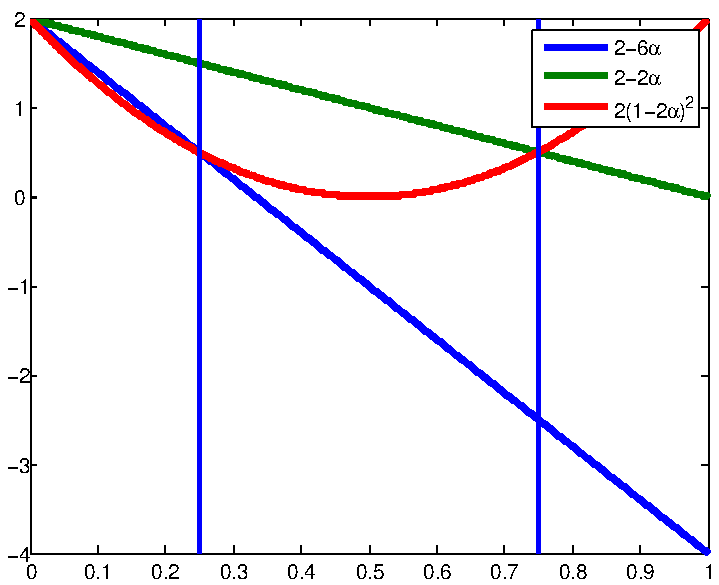
\includegraphics[width=0.5\textwidth]{images/goldarmijo_cropped.pdf}
 \caption{Choosing a step length.}
\end{figure}

\end{example}

\subsection{Linear least squares} An important special case is when the function has the form
\begin{equation*}
 f(\vct{x}) = \frac{1}{2}\norm{\mtx{A}\vct{x}-\vct{b}}_2^2.
\end{equation*}
Recall from Problem (1.5) that the Hessian is symmetric and positive semidefinite, with the gradient given by
\begin{equation*}
 \nabla f(\vct{x}) = \mtx{A}^{\trans}(\mtx{A}\vct{x}-\vct{b}).
\end{equation*}
The method of gradient descent proceeds as
\begin{equation*}
 \vct{x}_{k+1} = \vct{x}_k-\alpha_k \mtx{A}^{\top}(\mtx{A}\vct{x}_k-\vct{b}).
\end{equation*}
To find the best $\alpha_k$, we compute the minimum of the function
\begin{equation}\label{eq:minalpha}
 \alpha \mapsto f(\vct{x}+\alpha \mtx{A}^{\trans}(\vct{b}-\mtx{A}\vct{x})).
\end{equation}
If we set $\vct{r}:=\mtx{A}^{\trans}(\vct{b}-\mtx{A}\vct{x})$ and compute the minimum of~\eqref{eq:minalpha} by differentiating, we get the step length
\begin{equation*}
 \alpha = \frac{\vct{r}^{\trans}\vct{r}}{\vct{r}^{\trans}\mtx{A}^\trans\mtx{A}\vct{r}}.
\end{equation*}
The gradient descent algorithm for the linear least squares problem proceeds by first computing $\vct{r}_0=\mtx{A}^{\trans}(\vct{b}-\mtx{A}\vct{x}_0)$, and then at each step
\begin{align*}
 \alpha_k &= \frac{\vct{r}_k^{\trans}\vct{r}_k}{\vct{r}_k^{\trans}\mtx{A}^\trans\mtx{A}\vct{r}_k}\\
 \vct{x}_{k+1} &= \vct{x}_k+\alpha_k \vct{r}_k\\
 \vct{r}_{k+1} &= \vct{r}_k - \alpha_{k}\mtx{A}^{\trans}\mtx{A}\vct{r}_k.
\end{align*}
Does this work? How do we know when to stop? It is worth noting that the residual satisfies $\vct{r}=0$ if and only if $\vct{x}$ is a stationary point, in our case, a minimizer. One criteria for stopping could then be to check whether $\norm{\vct{r}_k}_2\leq \e$ for some given tolerance $\e>0$.

\begin{example}
 We test this method with the linear regression problem from Lecture 1, where we determinded the relationship $Y=\beta_0+\beta_1X$ of adult mass to basal metabolic rate in mammals. In this example, the matrix $\mtx{A}$ is the $2\times 573$ matrix
 \begin{equation*}
  \mtx{A} = \begin{pmatrix}
             1 & x_1\\
             \vdots & \vdots\\
             1 & x_{573}
            \end{pmatrix},
            \end{equation*}
where the $x_i$ represent the mass of mammal $i$, and the vector $\vct{b}$ consists of the metabolic rate parameters. The $2$-vector $\vct{x}$ represents the two values $\beta_0$ and $\beta_1$. A naive MATLAB code for gradient descent looks as follows.
\begin{lstlisting}
function xout = graddesc(A,b,x,tol)
    r = A'*(b-A*x);
    while norm(r,2)>tol
        Ar = A*r;
        alpha = r'*r/(Ar'*Ar);
        x = x+alpha*r;
        r = r-alpha*A'*Ar;
    end
    xout = x;
end
\end{lstlisting}
The result is the same as when using the MATLAB solver or CVX,
$\beta_0 = 1.36$, $\beta_1 = 0.70$.
\end{example}


In the next lecture we will introduce the concept of rate of convergence and analyse the rate of convergence of gradient descent.

%-----------------------------------------------------------------------
% End of chap1.tex
%-----------------------------------------------------------------------


%\appendix
%\include{appendix1}

%\backmatter
%\include{biblio}
%\include{index}
\end{document}

%-----------------------------------------------------------------------
% End of chapter.tex
%-----------------------------------------------------------------------
